The hadronic reaction to study is deep-inelastic lepton-proton scattering:
\begin{equation}
\Pleptonminus(l_1) + \Pp(p) \rightarrow \Pleptonminus(l_2) + \PQ(p_1)(\PaQ(p_2)) + X
\end{equation}
where one either detects the heavy quark $\PQ$ \textit{or} the heavy antiquark $\PaQ$ and $X$ stands for any final hadronic state allowed by quantum-number conservation. We define then the hadronic Bjorken variables
\begin{equation}
q=l_1-l_2, \quad Q^2=-q^2, \quad x=\frac{Q^2}{2p\cdot q}, \quad z = \frac{p\cdot q}{p\cdot l_1}
\end{equation}

We can then define the measurable deep-inelastic hadron structure functions
\begin{align}
F_k(x,Q^2,m^2) &= \sum_{n=0}^\infty F_{k}^{(n)}(x,Q^2,m^2)\\
F_{k}^{(n)}(x,Q^2,m^2) &= \frac{Q^2}{4\pi^2\alpha} \sum_{j\in\{\Pg,\Pq,\Paq\}}\int\limits_x^{z_{max}} \frac{dz}{z} f_j(x/z,\mu_F^2) \sigma^{(n)}_{k,j}(s,q^2,m^2)
\end{align}
where $k\in\{G,L,P\}$ denotes as usual projection, $z=Q^2/s'$, $z_{max} = Q^2/(4m^2+Q^2)$ and $f_j(x/z,\mu_F^2)$ denotes parton momentum density functions\cite{Martin:2009iq,PhysRevLett.113.012001}.
We can then split the contributions whether there is a gluon in the initial state $F_{k,g}$ or a (anti)quark $F_{k,q}$. In leading order we find:
\begin{align}
F_{k,g}^{(0)}(x,Q^2,m^2) &= \frac{\alpha_sQ^2}{4\pi^2m^2}e_H^2\int\limits_x^{z_{max}}\frac{dz}{z} f_g(x/z,\mu_F^2) c^{(0)}_{k,g}(\eta,\xi)
\end{align}
We find for the gluonic part in next-to-leading order:
\begin{align}
&F_{k,g}^{(1)}(x,Q^2,m^2) \nonumber\\
 &= \frac{\alpha_s^2Q^2}{\pi m^2}e_H^2\int\limits_x^{z_{max}}\frac{dz}{z} f_g(x/z,\mu_F^2) \left(c_{k,g}^{(1)}(\eta,\xi) + \ln(\mu_F^2/m^2)\bar c_{k,g}^{F,(1)}(\eta,\xi) + \ln(\mu_R^2/m^2)\bar c_{k,g}^{R,(1)}(\eta,\xi)\right)
\end{align}
We find for the quark part in next-to-leading order:
\begin{align}
&F_{k,q}^{(1)}(x,Q^2,m^2) \nonumber\\
 &= \frac{\alpha_s^2Q^2}{\pi m^2}e_H^2\int\limits_x^{z_{max}}\frac{dz}{z} \left(\sum_{j=1}^{n_{lf}}f_{q(j)}(x/z,\mu_F^2)+f_{q(-j)}(x/z,\mu_F^2)\right) \nonumber\\
 &\hspace{120pt} \cdot\left(c_{k,q}^{(1)}(\eta,\xi) + \ln(\mu_F^2/m^2)\bar c_{k,q}^{F,(1)}(\eta,\xi)\right) \nonumber\\
 &\hspace{20pt} + \frac{\alpha_s^2Q^2}{\pi m^2}\int\limits_x^{z_{max}}\frac{dz}{z} \left(\sum_{j=1}^{n_{lf}}e_{q(j)}^2\left(f_{q(j)}(x/z,\mu_F^2)+f_{q(-j)}(x/z,\mu_F^2)\right)\right) d_{k,q}(\eta,\xi)
\end{align}
where we used the PDG particle labeling\cite{Hagiwara:2002fs}: $q(1)=u,q(-1)=\bar u,q(2)=d,q(-2)=\bar d$, \ldots\,and $e_u = e_c = e_t = 2/3, e_d=e_s=e_b=-1/3$. 

We can then also define some more practical functions:
\begin{align}
F_{2}(x,Q^2,m^2) &= F_{T}(x,Q^2,m^2) + F_{L}(x,Q^2,m^2)\\
 &= F_{G}(x,Q^2,m^2) + \frac 3 2 F_{L}(x,Q^2,m^2)\\
F_1(x,Q^2,m^2) &= (F_{2}(x,Q^2,m^2)-F_L(x,Q^2,m^2))/(2x)\\
 &= \left(F_{G}(x,Q^2,m^2)+\frac 1 2 F_{L}(x,Q^2,m^2)\right)/(2x)\\
g_1(x,Q^2,m^2) &= F_{P}(x,Q^2,m^2)/(2x)
\end{align}
and we define
\begin{align}
R_{k'}(x,Q^2,m^2) &= \frac{F_{k'}^{(0)}(x,Q^2,m^2)+F_{k'}^{(1)}(x,Q^2,m^2)}{F_{k'}^{(0)}(x,Q^2,m^2)}
\end{align}
with $k'\in\{2,L,P\}$ to better observe next-to-leading order effects.

We define the spin asymmetry by
\begin{align}
A_1(x,Q^2,m^2) &= \frac{g_1(x,Q^2,m^2)}{F_1(x,Q^2,m^2)} = \frac{F_P(x,Q^2,m^2)}{F_2(x,Q^2,m^2)-F_L(x,Q^2,m^2)}
\end{align}

For the plots we focused on charm production ($n_{lf}=3$) with $m_c=\SI{1.5}{\GeV}$ and we used the two-loop running coupling of \cite{Altarelli:1988qr}:
\begin{align}
\alpha_s(\mu_R^2) &= \frac{1}{\beta_{0}^4\ln(\mu_R^2/\Lambda_4)}\left(1-\frac{\beta_1^4}{(\beta_0^4)^2} \ln(\ln(\mu_R^2/\Lambda_4))\right)
\end{align}
with the first two coefficients of the QCD beta function $\beta_0^f=(33-2f)/(12\pi)$ and $\beta_1^f=(306-38f)/(48\pi^2)$\fxerror{find CA?} and $\Lambda_4=\SI{0.194}{\GeV^2}$. We set $\mu_F^2=\mu_R^2=4m^2-q^2$ in analogy to \cite{Laenen1993162}. We used the PDF set MSTW2008nlo90cl\cite{Martin:2009iq,Martin:2009bu,Martin:2010db} provided by LHAPDF\cite{LHAPDF6} for the unpolarized structure functions ($F_2,F_1,F_G,F_L$) and DSSV2014\cite{PhysRevLett.113.012001} for the polarized structure function ($g_1,F_G$).

\fxerror{shift images to appendix?}

\begin{figure}[ht!]
\centering
% GNUPLOT: LaTeX picture with Postscript
\begingroup
  \makeatletter
  \providecommand\color[2][]{%
    \GenericError{(gnuplot) \space\space\space\@spaces}{%
      Package color not loaded in conjunction with
      terminal option `colourtext'%
    }{See the gnuplot documentation for explanation.%
    }{Either use 'blacktext' in gnuplot or load the package
      color.sty in LaTeX.}%
    \renewcommand\color[2][]{}%
  }%
  \providecommand\includegraphics[2][]{%
    \GenericError{(gnuplot) \space\space\space\@spaces}{%
      Package graphicx or graphics not loaded%
    }{See the gnuplot documentation for explanation.%
    }{The gnuplot epslatex terminal needs graphicx.sty or graphics.sty.}%
    \renewcommand\includegraphics[2][]{}%
  }%
  \providecommand\rotatebox[2]{#2}%
  \@ifundefined{ifGPcolor}{%
    \newif\ifGPcolor
    \GPcolorfalse
  }{}%
  \@ifundefined{ifGPblacktext}{%
    \newif\ifGPblacktext
    \GPblacktexttrue
  }{}%
  % define a \g@addto@macro without @ in the name:
  \let\gplgaddtomacro\g@addto@macro
  % define empty templates for all commands taking text:
  \gdef\gplbacktext{}%
  \gdef\gplfronttext{}%
  \makeatother
  \ifGPblacktext
    % no textcolor at all
    \def\colorrgb#1{}%
    \def\colorgray#1{}%
  \else
    % gray or color?
    \ifGPcolor
      \def\colorrgb#1{\color[rgb]{#1}}%
      \def\colorgray#1{\color[gray]{#1}}%
      \expandafter\def\csname LTw\endcsname{\color{white}}%
      \expandafter\def\csname LTb\endcsname{\color{black}}%
      \expandafter\def\csname LTa\endcsname{\color{black}}%
      \expandafter\def\csname LT0\endcsname{\color[rgb]{1,0,0}}%
      \expandafter\def\csname LT1\endcsname{\color[rgb]{0,1,0}}%
      \expandafter\def\csname LT2\endcsname{\color[rgb]{0,0,1}}%
      \expandafter\def\csname LT3\endcsname{\color[rgb]{1,0,1}}%
      \expandafter\def\csname LT4\endcsname{\color[rgb]{0,1,1}}%
      \expandafter\def\csname LT5\endcsname{\color[rgb]{1,1,0}}%
      \expandafter\def\csname LT6\endcsname{\color[rgb]{0,0,0}}%
      \expandafter\def\csname LT7\endcsname{\color[rgb]{1,0.3,0}}%
      \expandafter\def\csname LT8\endcsname{\color[rgb]{0.5,0.5,0.5}}%
    \else
      % gray
      \def\colorrgb#1{\color{black}}%
      \def\colorgray#1{\color[gray]{#1}}%
      \expandafter\def\csname LTw\endcsname{\color{white}}%
      \expandafter\def\csname LTb\endcsname{\color{black}}%
      \expandafter\def\csname LTa\endcsname{\color{black}}%
      \expandafter\def\csname LT0\endcsname{\color{black}}%
      \expandafter\def\csname LT1\endcsname{\color{black}}%
      \expandafter\def\csname LT2\endcsname{\color{black}}%
      \expandafter\def\csname LT3\endcsname{\color{black}}%
      \expandafter\def\csname LT4\endcsname{\color{black}}%
      \expandafter\def\csname LT5\endcsname{\color{black}}%
      \expandafter\def\csname LT6\endcsname{\color{black}}%
      \expandafter\def\csname LT7\endcsname{\color{black}}%
      \expandafter\def\csname LT8\endcsname{\color{black}}%
    \fi
  \fi
    \setlength{\unitlength}{0.0500bp}%
    \ifx\gptboxheight\undefined%
      \newlength{\gptboxheight}%
      \newlength{\gptboxwidth}%
      \newsavebox{\gptboxtext}%
    \fi%
    \setlength{\fboxrule}{0.5pt}%
    \setlength{\fboxsep}{1pt}%
\begin{picture}(7920.00,5040.00)%
    \gplgaddtomacro\gplbacktext{%
      \csname LTb\endcsname%
      \put(858,440){\makebox(0,0)[r]{\strut{}$-0.05$}}%
      \put(858,982){\makebox(0,0)[r]{\strut{}$0$}}%
      \put(858,1524){\makebox(0,0)[r]{\strut{}$0.05$}}%
      \put(858,2066){\makebox(0,0)[r]{\strut{}$0.1$}}%
      \put(858,2608){\makebox(0,0)[r]{\strut{}$0.15$}}%
      \put(858,3149){\makebox(0,0)[r]{\strut{}$0.2$}}%
      \put(858,3691){\makebox(0,0)[r]{\strut{}$0.25$}}%
      \put(858,4233){\makebox(0,0)[r]{\strut{}$0.3$}}%
      \put(858,4775){\makebox(0,0)[r]{\strut{}$0.35$}}%
      \put(990,220){\makebox(0,0){\strut{}$0.0001$}}%
      \put(2623,220){\makebox(0,0){\strut{}$0.001$}}%
      \put(4256,220){\makebox(0,0){\strut{}$0.01$}}%
      \put(5889,220){\makebox(0,0){\strut{}$0.1$}}%
      \put(7522,220){\makebox(0,0){\strut{}$1$}}%
    }%
    \gplgaddtomacro\gplfronttext{%
      \csname LTb\endcsname%
      \put(1122,4602){\makebox(0,0)[l]{\strut{}$Q^2=10^{1}$, LO}}%
      \csname LTb\endcsname%
      \put(1122,4382){\makebox(0,0)[l]{\strut{}$Q^2=10^{1}$, LO+NLO}}%
      \csname LTb\endcsname%
      \put(1122,4162){\makebox(0,0)[l]{\strut{}$Q^2=10^{2}$, LO}}%
      \csname LTb\endcsname%
      \put(1122,3942){\makebox(0,0)[l]{\strut{}$Q^2=10^{2}$, LO+NLO}}%
    }%
    \gplbacktext
    \put(0,0){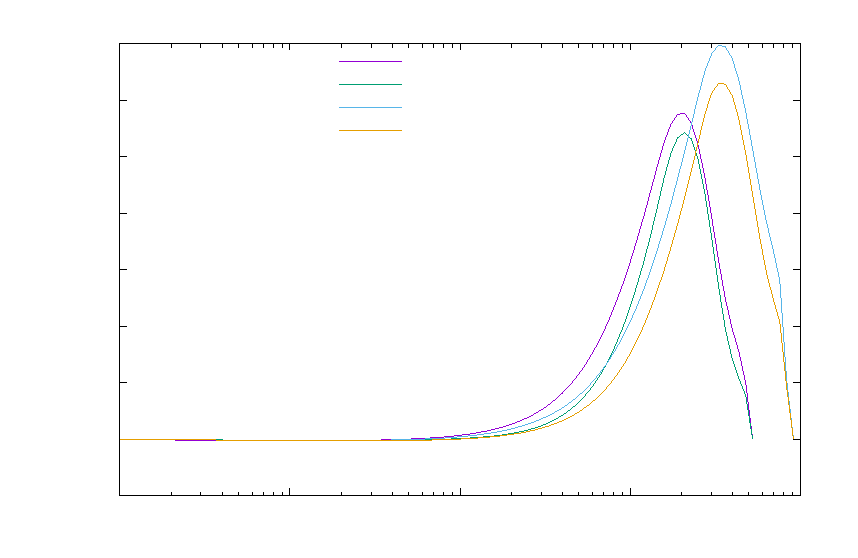
\includegraphics{img/A}}%
    \gplfronttext
  \end{picture}%
\endgroup

\caption{spin asymmetry $A_{1}(x,Q^2,m_c^2)$ plotted as function of $x$ for different values of $Q^2$ in units of $\si{\GeV^2}$}\label{fig:A}
\end{figure}

\pagebreak
\begin{figure}[ht!]
\centering
\begin{subfigure}[t]{\textwidth}
	% GNUPLOT: LaTeX picture with Postscript
\begingroup
  \makeatletter
  \providecommand\color[2][]{%
    \GenericError{(gnuplot) \space\space\space\@spaces}{%
      Package color not loaded in conjunction with
      terminal option `colourtext'%
    }{See the gnuplot documentation for explanation.%
    }{Either use 'blacktext' in gnuplot or load the package
      color.sty in LaTeX.}%
    \renewcommand\color[2][]{}%
  }%
  \providecommand\includegraphics[2][]{%
    \GenericError{(gnuplot) \space\space\space\@spaces}{%
      Package graphicx or graphics not loaded%
    }{See the gnuplot documentation for explanation.%
    }{The gnuplot epslatex terminal needs graphicx.sty or graphics.sty.}%
    \renewcommand\includegraphics[2][]{}%
  }%
  \providecommand\rotatebox[2]{#2}%
  \@ifundefined{ifGPcolor}{%
    \newif\ifGPcolor
    \GPcolorfalse
  }{}%
  \@ifundefined{ifGPblacktext}{%
    \newif\ifGPblacktext
    \GPblacktexttrue
  }{}%
  % define a \g@addto@macro without @ in the name:
  \let\gplgaddtomacro\g@addto@macro
  % define empty templates for all commands taking text:
  \gdef\gplbacktext{}%
  \gdef\gplfronttext{}%
  \makeatother
  \ifGPblacktext
    % no textcolor at all
    \def\colorrgb#1{}%
    \def\colorgray#1{}%
  \else
    % gray or color?
    \ifGPcolor
      \def\colorrgb#1{\color[rgb]{#1}}%
      \def\colorgray#1{\color[gray]{#1}}%
      \expandafter\def\csname LTw\endcsname{\color{white}}%
      \expandafter\def\csname LTb\endcsname{\color{black}}%
      \expandafter\def\csname LTa\endcsname{\color{black}}%
      \expandafter\def\csname LT0\endcsname{\color[rgb]{1,0,0}}%
      \expandafter\def\csname LT1\endcsname{\color[rgb]{0,1,0}}%
      \expandafter\def\csname LT2\endcsname{\color[rgb]{0,0,1}}%
      \expandafter\def\csname LT3\endcsname{\color[rgb]{1,0,1}}%
      \expandafter\def\csname LT4\endcsname{\color[rgb]{0,1,1}}%
      \expandafter\def\csname LT5\endcsname{\color[rgb]{1,1,0}}%
      \expandafter\def\csname LT6\endcsname{\color[rgb]{0,0,0}}%
      \expandafter\def\csname LT7\endcsname{\color[rgb]{1,0.3,0}}%
      \expandafter\def\csname LT8\endcsname{\color[rgb]{0.5,0.5,0.5}}%
    \else
      % gray
      \def\colorrgb#1{\color{black}}%
      \def\colorgray#1{\color[gray]{#1}}%
      \expandafter\def\csname LTw\endcsname{\color{white}}%
      \expandafter\def\csname LTb\endcsname{\color{black}}%
      \expandafter\def\csname LTa\endcsname{\color{black}}%
      \expandafter\def\csname LT0\endcsname{\color{black}}%
      \expandafter\def\csname LT1\endcsname{\color{black}}%
      \expandafter\def\csname LT2\endcsname{\color{black}}%
      \expandafter\def\csname LT3\endcsname{\color{black}}%
      \expandafter\def\csname LT4\endcsname{\color{black}}%
      \expandafter\def\csname LT5\endcsname{\color{black}}%
      \expandafter\def\csname LT6\endcsname{\color{black}}%
      \expandafter\def\csname LT7\endcsname{\color{black}}%
      \expandafter\def\csname LT8\endcsname{\color{black}}%
    \fi
  \fi
    \setlength{\unitlength}{0.0500bp}%
    \ifx\gptboxheight\undefined%
      \newlength{\gptboxheight}%
      \newlength{\gptboxwidth}%
      \newsavebox{\gptboxtext}%
    \fi%
    \setlength{\fboxrule}{0.5pt}%
    \setlength{\fboxsep}{1pt}%
\begin{picture}(7920.00,4082.40)%
    \gplgaddtomacro\gplbacktext{%
      \csname LTb\endcsname%
      \put(1254,220){\makebox(0,0)[r]{\strut{} 1.0e-06}}%
      \put(1254,820){\makebox(0,0)[r]{\strut{} 1.0e-05}}%
      \put(1254,1419){\makebox(0,0)[r]{\strut{} 1.0e-04}}%
      \put(1254,2019){\makebox(0,0)[r]{\strut{} 1.0e-03}}%
      \put(1254,2619){\makebox(0,0)[r]{\strut{} 1.0e-02}}%
      \put(1254,3218){\makebox(0,0)[r]{\strut{} 1.0e-01}}%
      \put(1254,3818){\makebox(0,0)[r]{\strut{} 1.0e+00}}%
      \put(1386,0){\makebox(0,0){\strut{}$0.0001$}}%
      \put(2920,0){\makebox(0,0){\strut{}$0.001$}}%
      \put(4454,0){\makebox(0,0){\strut{}$0.01$}}%
      \put(5988,0){\makebox(0,0){\strut{}$0.1$}}%
      \put(7522,0){\makebox(0,0){\strut{}$1$}}%
      \put(1509,2739){\makebox(0,0)[l]{\strut{}(a) $F_{2}(x,Q^2,m_c^2)$}}%
    }%
    \gplgaddtomacro\gplfronttext{%
      \csname LTb\endcsname%
      \put(1518,1053){\makebox(0,0)[l]{\strut{}$Q^2=10^{1}$, LO}}%
      \csname LTb\endcsname%
      \put(1518,833){\makebox(0,0)[l]{\strut{}$Q^2=10^{1}$, LO+NLO}}%
      \csname LTb\endcsname%
      \put(1518,613){\makebox(0,0)[l]{\strut{}$Q^2=10^{2}$, LO}}%
      \csname LTb\endcsname%
      \put(1518,393){\makebox(0,0)[l]{\strut{}$Q^2=10^{2}$, LO+NLO}}%
    }%
    \gplbacktext
    \put(0,0){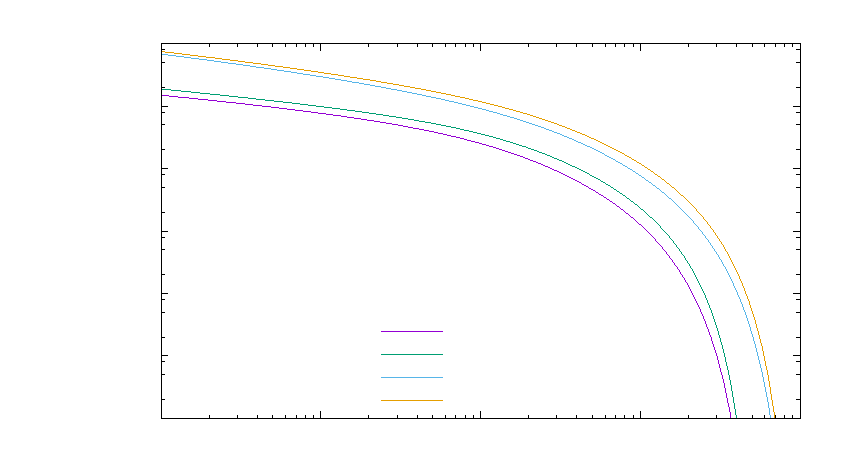
\includegraphics{img/F0012}}%
    \gplfronttext
  \end{picture}%
\endgroup

\end{subfigure}\\%
\begin{subfigure}[t]{\textwidth}
	% GNUPLOT: LaTeX picture with Postscript
\begingroup
  \makeatletter
  \providecommand\color[2][]{%
    \GenericError{(gnuplot) \space\space\space\@spaces}{%
      Package color not loaded in conjunction with
      terminal option `colourtext'%
    }{See the gnuplot documentation for explanation.%
    }{Either use 'blacktext' in gnuplot or load the package
      color.sty in LaTeX.}%
    \renewcommand\color[2][]{}%
  }%
  \providecommand\includegraphics[2][]{%
    \GenericError{(gnuplot) \space\space\space\@spaces}{%
      Package graphicx or graphics not loaded%
    }{See the gnuplot documentation for explanation.%
    }{The gnuplot epslatex terminal needs graphicx.sty or graphics.sty.}%
    \renewcommand\includegraphics[2][]{}%
  }%
  \providecommand\rotatebox[2]{#2}%
  \@ifundefined{ifGPcolor}{%
    \newif\ifGPcolor
    \GPcolorfalse
  }{}%
  \@ifundefined{ifGPblacktext}{%
    \newif\ifGPblacktext
    \GPblacktexttrue
  }{}%
  % define a \g@addto@macro without @ in the name:
  \let\gplgaddtomacro\g@addto@macro
  % define empty templates for all commands taking text:
  \gdef\gplbacktext{}%
  \gdef\gplfronttext{}%
  \makeatother
  \ifGPblacktext
    % no textcolor at all
    \def\colorrgb#1{}%
    \def\colorgray#1{}%
  \else
    % gray or color?
    \ifGPcolor
      \def\colorrgb#1{\color[rgb]{#1}}%
      \def\colorgray#1{\color[gray]{#1}}%
      \expandafter\def\csname LTw\endcsname{\color{white}}%
      \expandafter\def\csname LTb\endcsname{\color{black}}%
      \expandafter\def\csname LTa\endcsname{\color{black}}%
      \expandafter\def\csname LT0\endcsname{\color[rgb]{1,0,0}}%
      \expandafter\def\csname LT1\endcsname{\color[rgb]{0,1,0}}%
      \expandafter\def\csname LT2\endcsname{\color[rgb]{0,0,1}}%
      \expandafter\def\csname LT3\endcsname{\color[rgb]{1,0,1}}%
      \expandafter\def\csname LT4\endcsname{\color[rgb]{0,1,1}}%
      \expandafter\def\csname LT5\endcsname{\color[rgb]{1,1,0}}%
      \expandafter\def\csname LT6\endcsname{\color[rgb]{0,0,0}}%
      \expandafter\def\csname LT7\endcsname{\color[rgb]{1,0.3,0}}%
      \expandafter\def\csname LT8\endcsname{\color[rgb]{0.5,0.5,0.5}}%
    \else
      % gray
      \def\colorrgb#1{\color{black}}%
      \def\colorgray#1{\color[gray]{#1}}%
      \expandafter\def\csname LTw\endcsname{\color{white}}%
      \expandafter\def\csname LTb\endcsname{\color{black}}%
      \expandafter\def\csname LTa\endcsname{\color{black}}%
      \expandafter\def\csname LT0\endcsname{\color{black}}%
      \expandafter\def\csname LT1\endcsname{\color{black}}%
      \expandafter\def\csname LT2\endcsname{\color{black}}%
      \expandafter\def\csname LT3\endcsname{\color{black}}%
      \expandafter\def\csname LT4\endcsname{\color{black}}%
      \expandafter\def\csname LT5\endcsname{\color{black}}%
      \expandafter\def\csname LT6\endcsname{\color{black}}%
      \expandafter\def\csname LT7\endcsname{\color{black}}%
      \expandafter\def\csname LT8\endcsname{\color{black}}%
    \fi
  \fi
    \setlength{\unitlength}{0.0500bp}%
    \ifx\gptboxheight\undefined%
      \newlength{\gptboxheight}%
      \newlength{\gptboxwidth}%
      \newsavebox{\gptboxtext}%
    \fi%
    \setlength{\fboxrule}{0.5pt}%
    \setlength{\fboxsep}{1pt}%
\begin{picture}(7920.00,4082.40)%
    \gplgaddtomacro\gplbacktext{%
      \csname LTb\endcsname%
      \put(1254,220){\makebox(0,0)[r]{\strut{} 1.0e-06}}%
      \put(1254,820){\makebox(0,0)[r]{\strut{} 1.0e-05}}%
      \put(1254,1419){\makebox(0,0)[r]{\strut{} 1.0e-04}}%
      \put(1254,2019){\makebox(0,0)[r]{\strut{} 1.0e-03}}%
      \put(1254,2619){\makebox(0,0)[r]{\strut{} 1.0e-02}}%
      \put(1254,3218){\makebox(0,0)[r]{\strut{} 1.0e-01}}%
      \put(1254,3818){\makebox(0,0)[r]{\strut{} 1.0e+00}}%
      \put(1386,0){\makebox(0,0){\strut{}$0.0001$}}%
      \put(2920,0){\makebox(0,0){\strut{}$0.001$}}%
      \put(4454,0){\makebox(0,0){\strut{}$0.01$}}%
      \put(5988,0){\makebox(0,0){\strut{}$0.1$}}%
      \put(7522,0){\makebox(0,0){\strut{}$1$}}%
      \put(1509,3530){\makebox(0,0)[l]{\strut{}(b) $F_{L}(x,Q^2,m_c^2)$}}%
    }%
    \gplgaddtomacro\gplfronttext{%
      \csname LTb\endcsname%
      \put(1518,1053){\makebox(0,0)[l]{\strut{}$Q^2=10^{1}$, LO}}%
      \csname LTb\endcsname%
      \put(1518,833){\makebox(0,0)[l]{\strut{}$Q^2=10^{1}$, LO+NLO}}%
      \csname LTb\endcsname%
      \put(1518,613){\makebox(0,0)[l]{\strut{}$Q^2=10^{2}$, LO}}%
      \csname LTb\endcsname%
      \put(1518,393){\makebox(0,0)[l]{\strut{}$Q^2=10^{2}$, LO+NLO}}%
    }%
    \gplbacktext
    \put(0,0){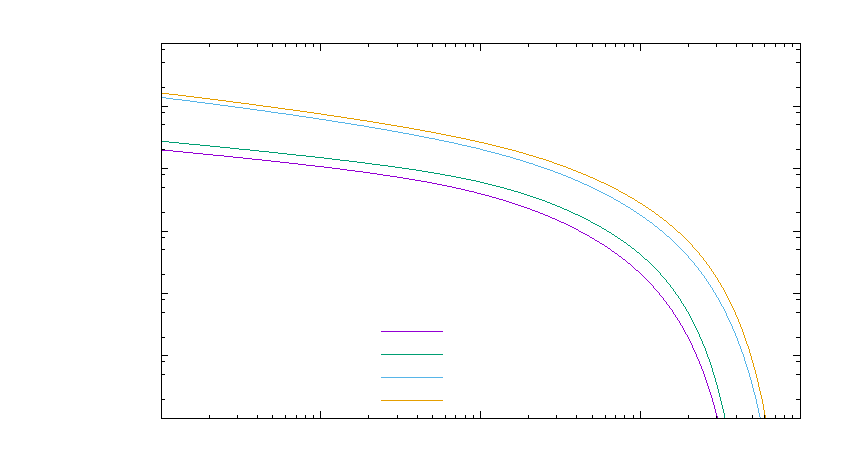
\includegraphics{img/F001L}}%
    \gplfronttext
  \end{picture}%
\endgroup

\end{subfigure}\\%
\begin{subfigure}[t]{\textwidth}
	% GNUPLOT: LaTeX picture with Postscript
\begingroup
  \makeatletter
  \providecommand\color[2][]{%
    \GenericError{(gnuplot) \space\space\space\@spaces}{%
      Package color not loaded in conjunction with
      terminal option `colourtext'%
    }{See the gnuplot documentation for explanation.%
    }{Either use 'blacktext' in gnuplot or load the package
      color.sty in LaTeX.}%
    \renewcommand\color[2][]{}%
  }%
  \providecommand\includegraphics[2][]{%
    \GenericError{(gnuplot) \space\space\space\@spaces}{%
      Package graphicx or graphics not loaded%
    }{See the gnuplot documentation for explanation.%
    }{The gnuplot epslatex terminal needs graphicx.sty or graphics.sty.}%
    \renewcommand\includegraphics[2][]{}%
  }%
  \providecommand\rotatebox[2]{#2}%
  \@ifundefined{ifGPcolor}{%
    \newif\ifGPcolor
    \GPcolorfalse
  }{}%
  \@ifundefined{ifGPblacktext}{%
    \newif\ifGPblacktext
    \GPblacktexttrue
  }{}%
  % define a \g@addto@macro without @ in the name:
  \let\gplgaddtomacro\g@addto@macro
  % define empty templates for all commands taking text:
  \gdef\gplbacktext{}%
  \gdef\gplfronttext{}%
  \makeatother
  \ifGPblacktext
    % no textcolor at all
    \def\colorrgb#1{}%
    \def\colorgray#1{}%
  \else
    % gray or color?
    \ifGPcolor
      \def\colorrgb#1{\color[rgb]{#1}}%
      \def\colorgray#1{\color[gray]{#1}}%
      \expandafter\def\csname LTw\endcsname{\color{white}}%
      \expandafter\def\csname LTb\endcsname{\color{black}}%
      \expandafter\def\csname LTa\endcsname{\color{black}}%
      \expandafter\def\csname LT0\endcsname{\color[rgb]{1,0,0}}%
      \expandafter\def\csname LT1\endcsname{\color[rgb]{0,1,0}}%
      \expandafter\def\csname LT2\endcsname{\color[rgb]{0,0,1}}%
      \expandafter\def\csname LT3\endcsname{\color[rgb]{1,0,1}}%
      \expandafter\def\csname LT4\endcsname{\color[rgb]{0,1,1}}%
      \expandafter\def\csname LT5\endcsname{\color[rgb]{1,1,0}}%
      \expandafter\def\csname LT6\endcsname{\color[rgb]{0,0,0}}%
      \expandafter\def\csname LT7\endcsname{\color[rgb]{1,0.3,0}}%
      \expandafter\def\csname LT8\endcsname{\color[rgb]{0.5,0.5,0.5}}%
    \else
      % gray
      \def\colorrgb#1{\color{black}}%
      \def\colorgray#1{\color[gray]{#1}}%
      \expandafter\def\csname LTw\endcsname{\color{white}}%
      \expandafter\def\csname LTb\endcsname{\color{black}}%
      \expandafter\def\csname LTa\endcsname{\color{black}}%
      \expandafter\def\csname LT0\endcsname{\color{black}}%
      \expandafter\def\csname LT1\endcsname{\color{black}}%
      \expandafter\def\csname LT2\endcsname{\color{black}}%
      \expandafter\def\csname LT3\endcsname{\color{black}}%
      \expandafter\def\csname LT4\endcsname{\color{black}}%
      \expandafter\def\csname LT5\endcsname{\color{black}}%
      \expandafter\def\csname LT6\endcsname{\color{black}}%
      \expandafter\def\csname LT7\endcsname{\color{black}}%
      \expandafter\def\csname LT8\endcsname{\color{black}}%
    \fi
  \fi
    \setlength{\unitlength}{0.0500bp}%
    \ifx\gptboxheight\undefined%
      \newlength{\gptboxheight}%
      \newlength{\gptboxwidth}%
      \newsavebox{\gptboxtext}%
    \fi%
    \setlength{\fboxrule}{0.5pt}%
    \setlength{\fboxsep}{1pt}%
\begin{picture}(7920.00,4082.40)%
    \gplgaddtomacro\gplbacktext{%
      \csname LTb\endcsname%
      \put(1254,220){\makebox(0,0)[r]{\strut{}-4.0e-04}}%
      \put(1254,820){\makebox(0,0)[r]{\strut{}-2.0e-04}}%
      \put(1254,1419){\makebox(0,0)[r]{\strut{}0.0e+00}}%
      \put(1254,2019){\makebox(0,0)[r]{\strut{}2.0e-04}}%
      \put(1254,2619){\makebox(0,0)[r]{\strut{}4.0e-04}}%
      \put(1254,3218){\makebox(0,0)[r]{\strut{}6.0e-04}}%
      \put(1254,3818){\makebox(0,0)[r]{\strut{}8.0e-04}}%
      \put(1386,0){\makebox(0,0){\strut{}$0.0001$}}%
      \put(2920,0){\makebox(0,0){\strut{}$0.001$}}%
      \put(4454,0){\makebox(0,0){\strut{}$0.01$}}%
      \put(5988,0){\makebox(0,0){\strut{}$0.1$}}%
      \put(7522,0){\makebox(0,0){\strut{}$1$}}%
      \put(1509,3530){\makebox(0,0)[l]{\strut{}(c) $F_P(x,Q^2,m_c^2)$}}%
    }%
    \gplgaddtomacro\gplfronttext{%
      \csname LTb\endcsname%
      \put(4687,1053){\makebox(0,0)[l]{\strut{}$Q^2=10^{1}$, LO}}%
      \csname LTb\endcsname%
      \put(4687,833){\makebox(0,0)[l]{\strut{}$Q^2=10^{2}$, LO+NLO}}%
      \csname LTb\endcsname%
      \put(4687,613){\makebox(0,0)[l]{\strut{}$Q^2=10^{2}$, LO}}%
      \csname LTb\endcsname%
      \put(4687,393){\makebox(0,0)[l]{\strut{}$Q^2=10^{2}$, LO+NLO}}%
    }%
    \gplbacktext
    \put(0,0){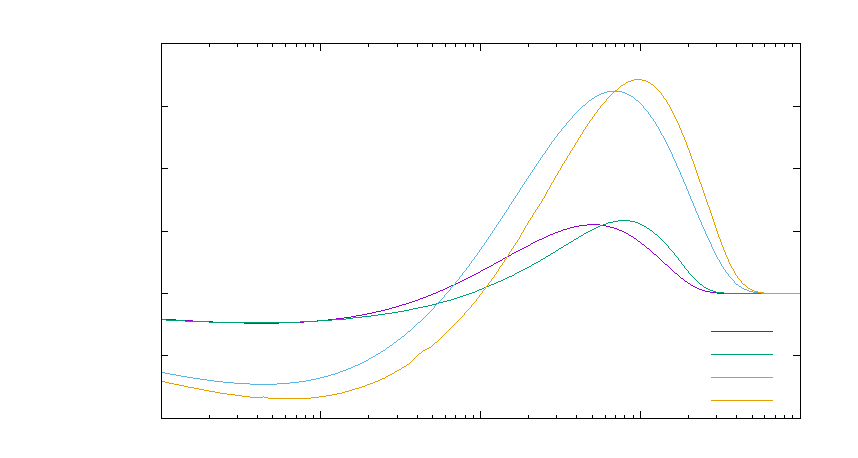
\includegraphics{img/F001P}}%
    \gplfronttext
  \end{picture}%
\endgroup

\end{subfigure}
\caption{hadronic structure functions $F_{k}(x,Q^2,m_c^2)$ plotted as function of $x$ for different values of $Q^2$ in units of $\si{\GeV^2}$}\label{fig:F001}
\end{figure}

\pagebreak
\begin{figure}[ht!]
\centering
\begin{subfigure}[t]{\textwidth}
	% GNUPLOT: LaTeX picture with Postscript
\begingroup
  \makeatletter
  \providecommand\color[2][]{%
    \GenericError{(gnuplot) \space\space\space\@spaces}{%
      Package color not loaded in conjunction with
      terminal option `colourtext'%
    }{See the gnuplot documentation for explanation.%
    }{Either use 'blacktext' in gnuplot or load the package
      color.sty in LaTeX.}%
    \renewcommand\color[2][]{}%
  }%
  \providecommand\includegraphics[2][]{%
    \GenericError{(gnuplot) \space\space\space\@spaces}{%
      Package graphicx or graphics not loaded%
    }{See the gnuplot documentation for explanation.%
    }{The gnuplot epslatex terminal needs graphicx.sty or graphics.sty.}%
    \renewcommand\includegraphics[2][]{}%
  }%
  \providecommand\rotatebox[2]{#2}%
  \@ifundefined{ifGPcolor}{%
    \newif\ifGPcolor
    \GPcolorfalse
  }{}%
  \@ifundefined{ifGPblacktext}{%
    \newif\ifGPblacktext
    \GPblacktexttrue
  }{}%
  % define a \g@addto@macro without @ in the name:
  \let\gplgaddtomacro\g@addto@macro
  % define empty templates for all commands taking text:
  \gdef\gplbacktext{}%
  \gdef\gplfronttext{}%
  \makeatother
  \ifGPblacktext
    % no textcolor at all
    \def\colorrgb#1{}%
    \def\colorgray#1{}%
  \else
    % gray or color?
    \ifGPcolor
      \def\colorrgb#1{\color[rgb]{#1}}%
      \def\colorgray#1{\color[gray]{#1}}%
      \expandafter\def\csname LTw\endcsname{\color{white}}%
      \expandafter\def\csname LTb\endcsname{\color{black}}%
      \expandafter\def\csname LTa\endcsname{\color{black}}%
      \expandafter\def\csname LT0\endcsname{\color[rgb]{1,0,0}}%
      \expandafter\def\csname LT1\endcsname{\color[rgb]{0,1,0}}%
      \expandafter\def\csname LT2\endcsname{\color[rgb]{0,0,1}}%
      \expandafter\def\csname LT3\endcsname{\color[rgb]{1,0,1}}%
      \expandafter\def\csname LT4\endcsname{\color[rgb]{0,1,1}}%
      \expandafter\def\csname LT5\endcsname{\color[rgb]{1,1,0}}%
      \expandafter\def\csname LT6\endcsname{\color[rgb]{0,0,0}}%
      \expandafter\def\csname LT7\endcsname{\color[rgb]{1,0.3,0}}%
      \expandafter\def\csname LT8\endcsname{\color[rgb]{0.5,0.5,0.5}}%
    \else
      % gray
      \def\colorrgb#1{\color{black}}%
      \def\colorgray#1{\color[gray]{#1}}%
      \expandafter\def\csname LTw\endcsname{\color{white}}%
      \expandafter\def\csname LTb\endcsname{\color{black}}%
      \expandafter\def\csname LTa\endcsname{\color{black}}%
      \expandafter\def\csname LT0\endcsname{\color{black}}%
      \expandafter\def\csname LT1\endcsname{\color{black}}%
      \expandafter\def\csname LT2\endcsname{\color{black}}%
      \expandafter\def\csname LT3\endcsname{\color{black}}%
      \expandafter\def\csname LT4\endcsname{\color{black}}%
      \expandafter\def\csname LT5\endcsname{\color{black}}%
      \expandafter\def\csname LT6\endcsname{\color{black}}%
      \expandafter\def\csname LT7\endcsname{\color{black}}%
      \expandafter\def\csname LT8\endcsname{\color{black}}%
    \fi
  \fi
    \setlength{\unitlength}{0.0500bp}%
    \ifx\gptboxheight\undefined%
      \newlength{\gptboxheight}%
      \newlength{\gptboxwidth}%
      \newsavebox{\gptboxtext}%
    \fi%
    \setlength{\fboxrule}{0.5pt}%
    \setlength{\fboxsep}{1pt}%
\begin{picture}(7920.00,4082.40)%
    \gplgaddtomacro\gplbacktext{%
      \csname LTb\endcsname%
      \put(1254,220){\makebox(0,0)[r]{\strut{} 1.0e-06}}%
      \put(1254,820){\makebox(0,0)[r]{\strut{} 1.0e-05}}%
      \put(1254,1419){\makebox(0,0)[r]{\strut{} 1.0e-04}}%
      \put(1254,2019){\makebox(0,0)[r]{\strut{} 1.0e-03}}%
      \put(1254,2619){\makebox(0,0)[r]{\strut{} 1.0e-02}}%
      \put(1254,3218){\makebox(0,0)[r]{\strut{} 1.0e-01}}%
      \put(1254,3818){\makebox(0,0)[r]{\strut{} 1.0e+00}}%
      \put(1386,0){\makebox(0,0){\strut{}$0.0001$}}%
      \put(2920,0){\makebox(0,0){\strut{}$0.001$}}%
      \put(4454,0){\makebox(0,0){\strut{}$0.01$}}%
      \put(5988,0){\makebox(0,0){\strut{}$0.1$}}%
      \put(7522,0){\makebox(0,0){\strut{}$1$}}%
      \put(1509,3530){\makebox(0,0)[l]{\strut{}(a) $F_{2,g}^{(1)}(x,Q^2,m_c^2)$}}%
    }%
    \gplgaddtomacro\gplfronttext{%
      \csname LTb\endcsname%
      \put(1518,613){\makebox(0,0)[l]{\strut{}$Q^2=10^{1}$}}%
      \csname LTb\endcsname%
      \put(1518,393){\makebox(0,0)[l]{\strut{}$Q^2=10^{2}$}}%
    }%
    \gplbacktext
    \put(0,0){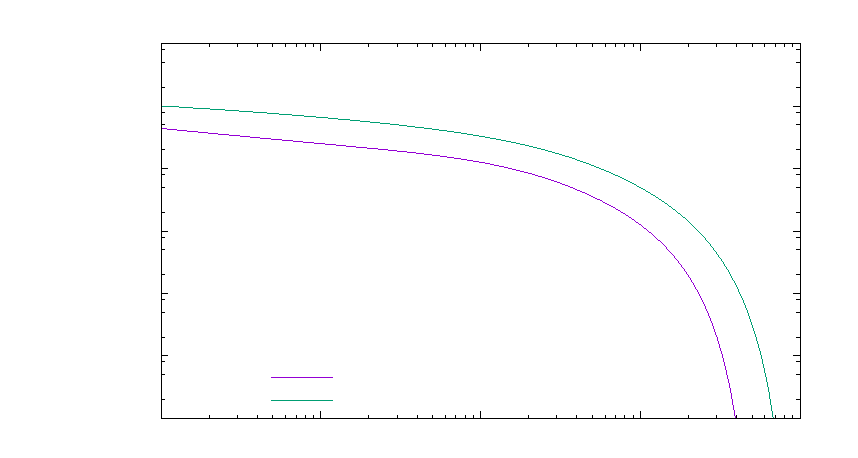
\includegraphics{img/Fg12}}%
    \gplfronttext
  \end{picture}%
\endgroup

\end{subfigure}\\%
\begin{subfigure}[t]{\textwidth}
	% GNUPLOT: LaTeX picture with Postscript
\begingroup
  \makeatletter
  \providecommand\color[2][]{%
    \GenericError{(gnuplot) \space\space\space\@spaces}{%
      Package color not loaded in conjunction with
      terminal option `colourtext'%
    }{See the gnuplot documentation for explanation.%
    }{Either use 'blacktext' in gnuplot or load the package
      color.sty in LaTeX.}%
    \renewcommand\color[2][]{}%
  }%
  \providecommand\includegraphics[2][]{%
    \GenericError{(gnuplot) \space\space\space\@spaces}{%
      Package graphicx or graphics not loaded%
    }{See the gnuplot documentation for explanation.%
    }{The gnuplot epslatex terminal needs graphicx.sty or graphics.sty.}%
    \renewcommand\includegraphics[2][]{}%
  }%
  \providecommand\rotatebox[2]{#2}%
  \@ifundefined{ifGPcolor}{%
    \newif\ifGPcolor
    \GPcolorfalse
  }{}%
  \@ifundefined{ifGPblacktext}{%
    \newif\ifGPblacktext
    \GPblacktexttrue
  }{}%
  % define a \g@addto@macro without @ in the name:
  \let\gplgaddtomacro\g@addto@macro
  % define empty templates for all commands taking text:
  \gdef\gplbacktext{}%
  \gdef\gplfronttext{}%
  \makeatother
  \ifGPblacktext
    % no textcolor at all
    \def\colorrgb#1{}%
    \def\colorgray#1{}%
  \else
    % gray or color?
    \ifGPcolor
      \def\colorrgb#1{\color[rgb]{#1}}%
      \def\colorgray#1{\color[gray]{#1}}%
      \expandafter\def\csname LTw\endcsname{\color{white}}%
      \expandafter\def\csname LTb\endcsname{\color{black}}%
      \expandafter\def\csname LTa\endcsname{\color{black}}%
      \expandafter\def\csname LT0\endcsname{\color[rgb]{1,0,0}}%
      \expandafter\def\csname LT1\endcsname{\color[rgb]{0,1,0}}%
      \expandafter\def\csname LT2\endcsname{\color[rgb]{0,0,1}}%
      \expandafter\def\csname LT3\endcsname{\color[rgb]{1,0,1}}%
      \expandafter\def\csname LT4\endcsname{\color[rgb]{0,1,1}}%
      \expandafter\def\csname LT5\endcsname{\color[rgb]{1,1,0}}%
      \expandafter\def\csname LT6\endcsname{\color[rgb]{0,0,0}}%
      \expandafter\def\csname LT7\endcsname{\color[rgb]{1,0.3,0}}%
      \expandafter\def\csname LT8\endcsname{\color[rgb]{0.5,0.5,0.5}}%
    \else
      % gray
      \def\colorrgb#1{\color{black}}%
      \def\colorgray#1{\color[gray]{#1}}%
      \expandafter\def\csname LTw\endcsname{\color{white}}%
      \expandafter\def\csname LTb\endcsname{\color{black}}%
      \expandafter\def\csname LTa\endcsname{\color{black}}%
      \expandafter\def\csname LT0\endcsname{\color{black}}%
      \expandafter\def\csname LT1\endcsname{\color{black}}%
      \expandafter\def\csname LT2\endcsname{\color{black}}%
      \expandafter\def\csname LT3\endcsname{\color{black}}%
      \expandafter\def\csname LT4\endcsname{\color{black}}%
      \expandafter\def\csname LT5\endcsname{\color{black}}%
      \expandafter\def\csname LT6\endcsname{\color{black}}%
      \expandafter\def\csname LT7\endcsname{\color{black}}%
      \expandafter\def\csname LT8\endcsname{\color{black}}%
    \fi
  \fi
    \setlength{\unitlength}{0.0500bp}%
    \ifx\gptboxheight\undefined%
      \newlength{\gptboxheight}%
      \newlength{\gptboxwidth}%
      \newsavebox{\gptboxtext}%
    \fi%
    \setlength{\fboxrule}{0.5pt}%
    \setlength{\fboxsep}{1pt}%
\begin{picture}(7920.00,4082.40)%
    \gplgaddtomacro\gplbacktext{%
      \csname LTb\endcsname%
      \put(1254,220){\makebox(0,0)[r]{\strut{} 1.0e-06}}%
      \put(1254,820){\makebox(0,0)[r]{\strut{} 1.0e-05}}%
      \put(1254,1419){\makebox(0,0)[r]{\strut{} 1.0e-04}}%
      \put(1254,2019){\makebox(0,0)[r]{\strut{} 1.0e-03}}%
      \put(1254,2619){\makebox(0,0)[r]{\strut{} 1.0e-02}}%
      \put(1254,3218){\makebox(0,0)[r]{\strut{} 1.0e-01}}%
      \put(1254,3818){\makebox(0,0)[r]{\strut{} 1.0e+00}}%
      \put(1386,0){\makebox(0,0){\strut{}$0.0001$}}%
      \put(2920,0){\makebox(0,0){\strut{}$0.001$}}%
      \put(4454,0){\makebox(0,0){\strut{}$0.01$}}%
      \put(5988,0){\makebox(0,0){\strut{}$0.1$}}%
      \put(7522,0){\makebox(0,0){\strut{}$1$}}%
      \put(1509,3530){\makebox(0,0)[l]{\strut{}(b) $F_{L,g}^{(1)}(x,Q^2,m_c^2)$}}%
    }%
    \gplgaddtomacro\gplfronttext{%
      \csname LTb\endcsname%
      \put(1518,613){\makebox(0,0)[l]{\strut{}$Q^2=10^{1}$}}%
      \csname LTb\endcsname%
      \put(1518,393){\makebox(0,0)[l]{\strut{}$Q^2=10^{2}$}}%
    }%
    \gplbacktext
    \put(0,0){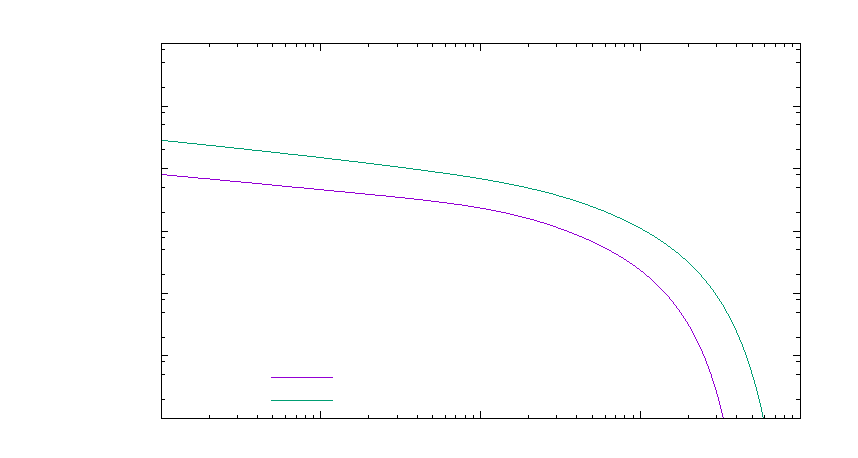
\includegraphics{img/Fg1L}}%
    \gplfronttext
  \end{picture}%
\endgroup

\end{subfigure}\\%
\begin{subfigure}[t]{\textwidth}
	% GNUPLOT: LaTeX picture with Postscript
\begingroup
  \makeatletter
  \providecommand\color[2][]{%
    \GenericError{(gnuplot) \space\space\space\@spaces}{%
      Package color not loaded in conjunction with
      terminal option `colourtext'%
    }{See the gnuplot documentation for explanation.%
    }{Either use 'blacktext' in gnuplot or load the package
      color.sty in LaTeX.}%
    \renewcommand\color[2][]{}%
  }%
  \providecommand\includegraphics[2][]{%
    \GenericError{(gnuplot) \space\space\space\@spaces}{%
      Package graphicx or graphics not loaded%
    }{See the gnuplot documentation for explanation.%
    }{The gnuplot epslatex terminal needs graphicx.sty or graphics.sty.}%
    \renewcommand\includegraphics[2][]{}%
  }%
  \providecommand\rotatebox[2]{#2}%
  \@ifundefined{ifGPcolor}{%
    \newif\ifGPcolor
    \GPcolorfalse
  }{}%
  \@ifundefined{ifGPblacktext}{%
    \newif\ifGPblacktext
    \GPblacktexttrue
  }{}%
  % define a \g@addto@macro without @ in the name:
  \let\gplgaddtomacro\g@addto@macro
  % define empty templates for all commands taking text:
  \gdef\gplbacktext{}%
  \gdef\gplfronttext{}%
  \makeatother
  \ifGPblacktext
    % no textcolor at all
    \def\colorrgb#1{}%
    \def\colorgray#1{}%
  \else
    % gray or color?
    \ifGPcolor
      \def\colorrgb#1{\color[rgb]{#1}}%
      \def\colorgray#1{\color[gray]{#1}}%
      \expandafter\def\csname LTw\endcsname{\color{white}}%
      \expandafter\def\csname LTb\endcsname{\color{black}}%
      \expandafter\def\csname LTa\endcsname{\color{black}}%
      \expandafter\def\csname LT0\endcsname{\color[rgb]{1,0,0}}%
      \expandafter\def\csname LT1\endcsname{\color[rgb]{0,1,0}}%
      \expandafter\def\csname LT2\endcsname{\color[rgb]{0,0,1}}%
      \expandafter\def\csname LT3\endcsname{\color[rgb]{1,0,1}}%
      \expandafter\def\csname LT4\endcsname{\color[rgb]{0,1,1}}%
      \expandafter\def\csname LT5\endcsname{\color[rgb]{1,1,0}}%
      \expandafter\def\csname LT6\endcsname{\color[rgb]{0,0,0}}%
      \expandafter\def\csname LT7\endcsname{\color[rgb]{1,0.3,0}}%
      \expandafter\def\csname LT8\endcsname{\color[rgb]{0.5,0.5,0.5}}%
    \else
      % gray
      \def\colorrgb#1{\color{black}}%
      \def\colorgray#1{\color[gray]{#1}}%
      \expandafter\def\csname LTw\endcsname{\color{white}}%
      \expandafter\def\csname LTb\endcsname{\color{black}}%
      \expandafter\def\csname LTa\endcsname{\color{black}}%
      \expandafter\def\csname LT0\endcsname{\color{black}}%
      \expandafter\def\csname LT1\endcsname{\color{black}}%
      \expandafter\def\csname LT2\endcsname{\color{black}}%
      \expandafter\def\csname LT3\endcsname{\color{black}}%
      \expandafter\def\csname LT4\endcsname{\color{black}}%
      \expandafter\def\csname LT5\endcsname{\color{black}}%
      \expandafter\def\csname LT6\endcsname{\color{black}}%
      \expandafter\def\csname LT7\endcsname{\color{black}}%
      \expandafter\def\csname LT8\endcsname{\color{black}}%
    \fi
  \fi
    \setlength{\unitlength}{0.0500bp}%
    \ifx\gptboxheight\undefined%
      \newlength{\gptboxheight}%
      \newlength{\gptboxwidth}%
      \newsavebox{\gptboxtext}%
    \fi%
    \setlength{\fboxrule}{0.5pt}%
    \setlength{\fboxsep}{1pt}%
\begin{picture}(7920.00,4082.40)%
    \gplgaddtomacro\gplbacktext{%
      \csname LTb\endcsname%
      \put(1254,220){\makebox(0,0)[r]{\strut{}-1.0e-04}}%
      \put(1254,670){\makebox(0,0)[r]{\strut{}-5.0e-05}}%
      \put(1254,1120){\makebox(0,0)[r]{\strut{}0.0e+00}}%
      \put(1254,1569){\makebox(0,0)[r]{\strut{}5.0e-05}}%
      \put(1254,2019){\makebox(0,0)[r]{\strut{}1.0e-04}}%
      \put(1254,2469){\makebox(0,0)[r]{\strut{}1.5e-04}}%
      \put(1254,2919){\makebox(0,0)[r]{\strut{}2.0e-04}}%
      \put(1254,3368){\makebox(0,0)[r]{\strut{}2.5e-04}}%
      \put(1254,3818){\makebox(0,0)[r]{\strut{}3.0e-04}}%
      \put(1386,0){\makebox(0,0){\strut{}$0.0001$}}%
      \put(2920,0){\makebox(0,0){\strut{}$0.001$}}%
      \put(4454,0){\makebox(0,0){\strut{}$0.01$}}%
      \put(5988,0){\makebox(0,0){\strut{}$0.1$}}%
      \put(7522,0){\makebox(0,0){\strut{}$1$}}%
      \put(1509,3530){\makebox(0,0)[l]{\strut{}(c) $F_{P,g}^{(1)}(x,Q^2,m_c^2)$}}%
    }%
    \gplgaddtomacro\gplfronttext{%
      \csname LTb\endcsname%
      \put(5743,613){\makebox(0,0)[l]{\strut{}$Q^2=10^{1}$}}%
      \csname LTb\endcsname%
      \put(5743,393){\makebox(0,0)[l]{\strut{}$Q^2=10^{2}$}}%
    }%
    \gplbacktext
    \put(0,0){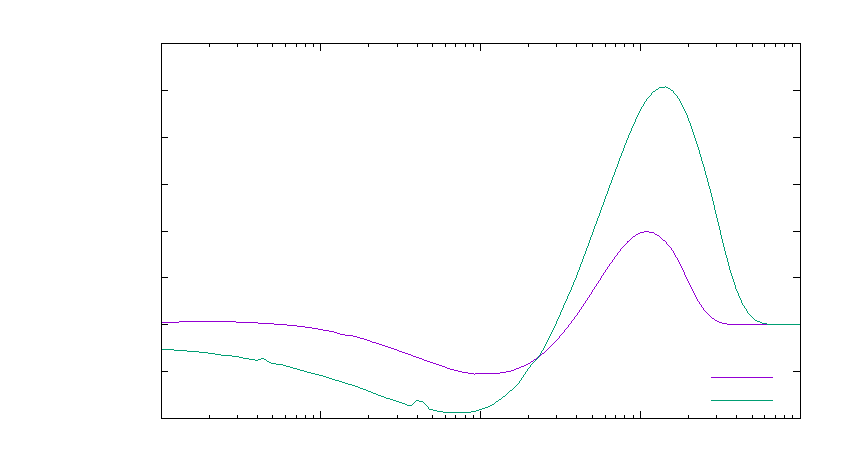
\includegraphics{img/Fg1P}}%
    \gplfronttext
  \end{picture}%
\endgroup

\end{subfigure}
\caption{next-to-leading order hadronic structure functions $F_{k,g}^{(1)}(x,Q^2,m_c^2)$ plotted as function of $x$ for different values of $Q^2$ in units of $\si{\GeV^2}$}\label{fig:Fg1}
\end{figure}

\pagebreak
\begin{figure}[ht!]
\centering
\begin{subfigure}[t]{\textwidth}
	% GNUPLOT: LaTeX picture with Postscript
\begingroup
  \makeatletter
  \providecommand\color[2][]{%
    \GenericError{(gnuplot) \space\space\space\@spaces}{%
      Package color not loaded in conjunction with
      terminal option `colourtext'%
    }{See the gnuplot documentation for explanation.%
    }{Either use 'blacktext' in gnuplot or load the package
      color.sty in LaTeX.}%
    \renewcommand\color[2][]{}%
  }%
  \providecommand\includegraphics[2][]{%
    \GenericError{(gnuplot) \space\space\space\@spaces}{%
      Package graphicx or graphics not loaded%
    }{See the gnuplot documentation for explanation.%
    }{The gnuplot epslatex terminal needs graphicx.sty or graphics.sty.}%
    \renewcommand\includegraphics[2][]{}%
  }%
  \providecommand\rotatebox[2]{#2}%
  \@ifundefined{ifGPcolor}{%
    \newif\ifGPcolor
    \GPcolorfalse
  }{}%
  \@ifundefined{ifGPblacktext}{%
    \newif\ifGPblacktext
    \GPblacktexttrue
  }{}%
  % define a \g@addto@macro without @ in the name:
  \let\gplgaddtomacro\g@addto@macro
  % define empty templates for all commands taking text:
  \gdef\gplbacktext{}%
  \gdef\gplfronttext{}%
  \makeatother
  \ifGPblacktext
    % no textcolor at all
    \def\colorrgb#1{}%
    \def\colorgray#1{}%
  \else
    % gray or color?
    \ifGPcolor
      \def\colorrgb#1{\color[rgb]{#1}}%
      \def\colorgray#1{\color[gray]{#1}}%
      \expandafter\def\csname LTw\endcsname{\color{white}}%
      \expandafter\def\csname LTb\endcsname{\color{black}}%
      \expandafter\def\csname LTa\endcsname{\color{black}}%
      \expandafter\def\csname LT0\endcsname{\color[rgb]{1,0,0}}%
      \expandafter\def\csname LT1\endcsname{\color[rgb]{0,1,0}}%
      \expandafter\def\csname LT2\endcsname{\color[rgb]{0,0,1}}%
      \expandafter\def\csname LT3\endcsname{\color[rgb]{1,0,1}}%
      \expandafter\def\csname LT4\endcsname{\color[rgb]{0,1,1}}%
      \expandafter\def\csname LT5\endcsname{\color[rgb]{1,1,0}}%
      \expandafter\def\csname LT6\endcsname{\color[rgb]{0,0,0}}%
      \expandafter\def\csname LT7\endcsname{\color[rgb]{1,0.3,0}}%
      \expandafter\def\csname LT8\endcsname{\color[rgb]{0.5,0.5,0.5}}%
    \else
      % gray
      \def\colorrgb#1{\color{black}}%
      \def\colorgray#1{\color[gray]{#1}}%
      \expandafter\def\csname LTw\endcsname{\color{white}}%
      \expandafter\def\csname LTb\endcsname{\color{black}}%
      \expandafter\def\csname LTa\endcsname{\color{black}}%
      \expandafter\def\csname LT0\endcsname{\color{black}}%
      \expandafter\def\csname LT1\endcsname{\color{black}}%
      \expandafter\def\csname LT2\endcsname{\color{black}}%
      \expandafter\def\csname LT3\endcsname{\color{black}}%
      \expandafter\def\csname LT4\endcsname{\color{black}}%
      \expandafter\def\csname LT5\endcsname{\color{black}}%
      \expandafter\def\csname LT6\endcsname{\color{black}}%
      \expandafter\def\csname LT7\endcsname{\color{black}}%
      \expandafter\def\csname LT8\endcsname{\color{black}}%
    \fi
  \fi
    \setlength{\unitlength}{0.0500bp}%
    \ifx\gptboxheight\undefined%
      \newlength{\gptboxheight}%
      \newlength{\gptboxwidth}%
      \newsavebox{\gptboxtext}%
    \fi%
    \setlength{\fboxrule}{0.5pt}%
    \setlength{\fboxsep}{1pt}%
\begin{picture}(7920.00,4082.40)%
    \gplgaddtomacro\gplbacktext{%
      \csname LTb\endcsname%
      \put(1254,220){\makebox(0,0)[r]{\strut{}-3.5e-02}}%
      \put(1254,734){\makebox(0,0)[r]{\strut{}-3.0e-02}}%
      \put(1254,1248){\makebox(0,0)[r]{\strut{}-2.5e-02}}%
      \put(1254,1762){\makebox(0,0)[r]{\strut{}-2.0e-02}}%
      \put(1254,2276){\makebox(0,0)[r]{\strut{}-1.5e-02}}%
      \put(1254,2790){\makebox(0,0)[r]{\strut{}-1.0e-02}}%
      \put(1254,3304){\makebox(0,0)[r]{\strut{}-5.0e-03}}%
      \put(1254,3818){\makebox(0,0)[r]{\strut{}0.0e+00}}%
      \put(1386,0){\makebox(0,0){\strut{}$0.0001$}}%
      \put(2920,0){\makebox(0,0){\strut{}$0.001$}}%
      \put(4454,0){\makebox(0,0){\strut{}$0.01$}}%
      \put(5988,0){\makebox(0,0){\strut{}$0.1$}}%
      \put(7522,0){\makebox(0,0){\strut{}$1$}}%
      \put(1509,2811){\makebox(0,0)[l]{\strut{}(a) $F_{2,q}^{(1)}(x,Q^2,m_c^2)$}}%
    }%
    \gplgaddtomacro\gplfronttext{%
      \csname LTb\endcsname%
      \put(5743,613){\makebox(0,0)[l]{\strut{}$Q^2=10^{1}$}}%
      \csname LTb\endcsname%
      \put(5743,393){\makebox(0,0)[l]{\strut{}$Q^2=10^{2}$}}%
    }%
    \gplbacktext
    \put(0,0){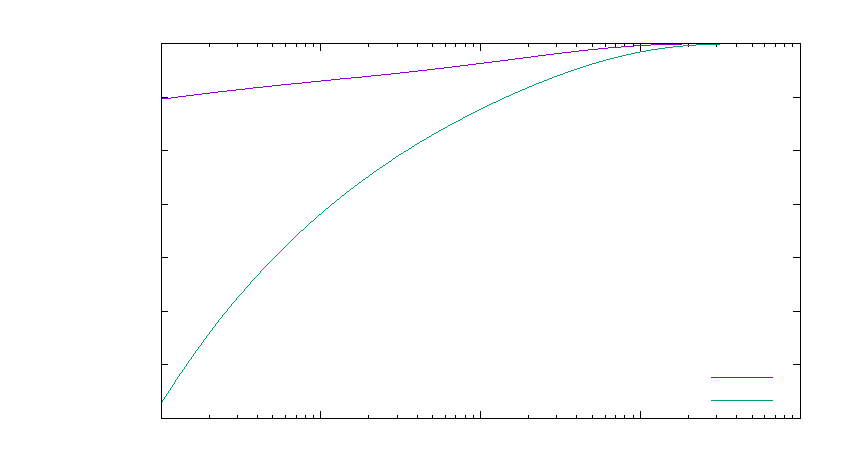
\includegraphics{img/Fq12}}%
    \gplfronttext
  \end{picture}%
\endgroup

\end{subfigure}\\%
\begin{subfigure}[t]{\textwidth}
	% GNUPLOT: LaTeX picture with Postscript
\begingroup
  \makeatletter
  \providecommand\color[2][]{%
    \GenericError{(gnuplot) \space\space\space\@spaces}{%
      Package color not loaded in conjunction with
      terminal option `colourtext'%
    }{See the gnuplot documentation for explanation.%
    }{Either use 'blacktext' in gnuplot or load the package
      color.sty in LaTeX.}%
    \renewcommand\color[2][]{}%
  }%
  \providecommand\includegraphics[2][]{%
    \GenericError{(gnuplot) \space\space\space\@spaces}{%
      Package graphicx or graphics not loaded%
    }{See the gnuplot documentation for explanation.%
    }{The gnuplot epslatex terminal needs graphicx.sty or graphics.sty.}%
    \renewcommand\includegraphics[2][]{}%
  }%
  \providecommand\rotatebox[2]{#2}%
  \@ifundefined{ifGPcolor}{%
    \newif\ifGPcolor
    \GPcolorfalse
  }{}%
  \@ifundefined{ifGPblacktext}{%
    \newif\ifGPblacktext
    \GPblacktexttrue
  }{}%
  % define a \g@addto@macro without @ in the name:
  \let\gplgaddtomacro\g@addto@macro
  % define empty templates for all commands taking text:
  \gdef\gplbacktext{}%
  \gdef\gplfronttext{}%
  \makeatother
  \ifGPblacktext
    % no textcolor at all
    \def\colorrgb#1{}%
    \def\colorgray#1{}%
  \else
    % gray or color?
    \ifGPcolor
      \def\colorrgb#1{\color[rgb]{#1}}%
      \def\colorgray#1{\color[gray]{#1}}%
      \expandafter\def\csname LTw\endcsname{\color{white}}%
      \expandafter\def\csname LTb\endcsname{\color{black}}%
      \expandafter\def\csname LTa\endcsname{\color{black}}%
      \expandafter\def\csname LT0\endcsname{\color[rgb]{1,0,0}}%
      \expandafter\def\csname LT1\endcsname{\color[rgb]{0,1,0}}%
      \expandafter\def\csname LT2\endcsname{\color[rgb]{0,0,1}}%
      \expandafter\def\csname LT3\endcsname{\color[rgb]{1,0,1}}%
      \expandafter\def\csname LT4\endcsname{\color[rgb]{0,1,1}}%
      \expandafter\def\csname LT5\endcsname{\color[rgb]{1,1,0}}%
      \expandafter\def\csname LT6\endcsname{\color[rgb]{0,0,0}}%
      \expandafter\def\csname LT7\endcsname{\color[rgb]{1,0.3,0}}%
      \expandafter\def\csname LT8\endcsname{\color[rgb]{0.5,0.5,0.5}}%
    \else
      % gray
      \def\colorrgb#1{\color{black}}%
      \def\colorgray#1{\color[gray]{#1}}%
      \expandafter\def\csname LTw\endcsname{\color{white}}%
      \expandafter\def\csname LTb\endcsname{\color{black}}%
      \expandafter\def\csname LTa\endcsname{\color{black}}%
      \expandafter\def\csname LT0\endcsname{\color{black}}%
      \expandafter\def\csname LT1\endcsname{\color{black}}%
      \expandafter\def\csname LT2\endcsname{\color{black}}%
      \expandafter\def\csname LT3\endcsname{\color{black}}%
      \expandafter\def\csname LT4\endcsname{\color{black}}%
      \expandafter\def\csname LT5\endcsname{\color{black}}%
      \expandafter\def\csname LT6\endcsname{\color{black}}%
      \expandafter\def\csname LT7\endcsname{\color{black}}%
      \expandafter\def\csname LT8\endcsname{\color{black}}%
    \fi
  \fi
    \setlength{\unitlength}{0.0500bp}%
    \ifx\gptboxheight\undefined%
      \newlength{\gptboxheight}%
      \newlength{\gptboxwidth}%
      \newsavebox{\gptboxtext}%
    \fi%
    \setlength{\fboxrule}{0.5pt}%
    \setlength{\fboxsep}{1pt}%
\begin{picture}(7920.00,4082.40)%
    \gplgaddtomacro\gplbacktext{%
      \csname LTb\endcsname%
      \put(1254,220){\makebox(0,0)[r]{\strut{}-4.0e-03}}%
      \put(1254,670){\makebox(0,0)[r]{\strut{}-3.5e-03}}%
      \put(1254,1120){\makebox(0,0)[r]{\strut{}-3.0e-03}}%
      \put(1254,1569){\makebox(0,0)[r]{\strut{}-2.5e-03}}%
      \put(1254,2019){\makebox(0,0)[r]{\strut{}-2.0e-03}}%
      \put(1254,2469){\makebox(0,0)[r]{\strut{}-1.5e-03}}%
      \put(1254,2919){\makebox(0,0)[r]{\strut{}-1.0e-03}}%
      \put(1254,3368){\makebox(0,0)[r]{\strut{}-5.0e-04}}%
      \put(1254,3818){\makebox(0,0)[r]{\strut{}0.0e+00}}%
      \put(1386,0){\makebox(0,0){\strut{}$0.0001$}}%
      \put(2920,0){\makebox(0,0){\strut{}$0.001$}}%
      \put(4454,0){\makebox(0,0){\strut{}$0.01$}}%
      \put(5988,0){\makebox(0,0){\strut{}$0.1$}}%
      \put(7522,0){\makebox(0,0){\strut{}$1$}}%
      \put(1509,2811){\makebox(0,0)[l]{\strut{}(b) $F_{L,q}^{(1)}(x,Q^2,m_c^2)$}}%
    }%
    \gplgaddtomacro\gplfronttext{%
      \csname LTb\endcsname%
      \put(5743,613){\makebox(0,0)[l]{\strut{}$Q^2=10^{1}$}}%
      \csname LTb\endcsname%
      \put(5743,393){\makebox(0,0)[l]{\strut{}$Q^2=10^{2}$}}%
    }%
    \gplbacktext
    \put(0,0){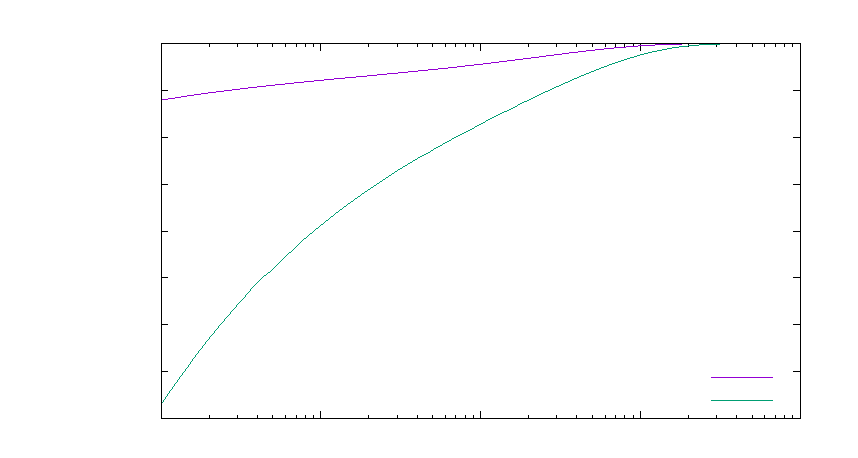
\includegraphics{img/Fq1L}}%
    \gplfronttext
  \end{picture}%
\endgroup

\end{subfigure}\\%
\begin{subfigure}[t]{\textwidth}
	% GNUPLOT: LaTeX picture with Postscript
\begingroup
  \makeatletter
  \providecommand\color[2][]{%
    \GenericError{(gnuplot) \space\space\space\@spaces}{%
      Package color not loaded in conjunction with
      terminal option `colourtext'%
    }{See the gnuplot documentation for explanation.%
    }{Either use 'blacktext' in gnuplot or load the package
      color.sty in LaTeX.}%
    \renewcommand\color[2][]{}%
  }%
  \providecommand\includegraphics[2][]{%
    \GenericError{(gnuplot) \space\space\space\@spaces}{%
      Package graphicx or graphics not loaded%
    }{See the gnuplot documentation for explanation.%
    }{The gnuplot epslatex terminal needs graphicx.sty or graphics.sty.}%
    \renewcommand\includegraphics[2][]{}%
  }%
  \providecommand\rotatebox[2]{#2}%
  \@ifundefined{ifGPcolor}{%
    \newif\ifGPcolor
    \GPcolorfalse
  }{}%
  \@ifundefined{ifGPblacktext}{%
    \newif\ifGPblacktext
    \GPblacktexttrue
  }{}%
  % define a \g@addto@macro without @ in the name:
  \let\gplgaddtomacro\g@addto@macro
  % define empty templates for all commands taking text:
  \gdef\gplbacktext{}%
  \gdef\gplfronttext{}%
  \makeatother
  \ifGPblacktext
    % no textcolor at all
    \def\colorrgb#1{}%
    \def\colorgray#1{}%
  \else
    % gray or color?
    \ifGPcolor
      \def\colorrgb#1{\color[rgb]{#1}}%
      \def\colorgray#1{\color[gray]{#1}}%
      \expandafter\def\csname LTw\endcsname{\color{white}}%
      \expandafter\def\csname LTb\endcsname{\color{black}}%
      \expandafter\def\csname LTa\endcsname{\color{black}}%
      \expandafter\def\csname LT0\endcsname{\color[rgb]{1,0,0}}%
      \expandafter\def\csname LT1\endcsname{\color[rgb]{0,1,0}}%
      \expandafter\def\csname LT2\endcsname{\color[rgb]{0,0,1}}%
      \expandafter\def\csname LT3\endcsname{\color[rgb]{1,0,1}}%
      \expandafter\def\csname LT4\endcsname{\color[rgb]{0,1,1}}%
      \expandafter\def\csname LT5\endcsname{\color[rgb]{1,1,0}}%
      \expandafter\def\csname LT6\endcsname{\color[rgb]{0,0,0}}%
      \expandafter\def\csname LT7\endcsname{\color[rgb]{1,0.3,0}}%
      \expandafter\def\csname LT8\endcsname{\color[rgb]{0.5,0.5,0.5}}%
    \else
      % gray
      \def\colorrgb#1{\color{black}}%
      \def\colorgray#1{\color[gray]{#1}}%
      \expandafter\def\csname LTw\endcsname{\color{white}}%
      \expandafter\def\csname LTb\endcsname{\color{black}}%
      \expandafter\def\csname LTa\endcsname{\color{black}}%
      \expandafter\def\csname LT0\endcsname{\color{black}}%
      \expandafter\def\csname LT1\endcsname{\color{black}}%
      \expandafter\def\csname LT2\endcsname{\color{black}}%
      \expandafter\def\csname LT3\endcsname{\color{black}}%
      \expandafter\def\csname LT4\endcsname{\color{black}}%
      \expandafter\def\csname LT5\endcsname{\color{black}}%
      \expandafter\def\csname LT6\endcsname{\color{black}}%
      \expandafter\def\csname LT7\endcsname{\color{black}}%
      \expandafter\def\csname LT8\endcsname{\color{black}}%
    \fi
  \fi
    \setlength{\unitlength}{0.0500bp}%
    \ifx\gptboxheight\undefined%
      \newlength{\gptboxheight}%
      \newlength{\gptboxwidth}%
      \newsavebox{\gptboxtext}%
    \fi%
    \setlength{\fboxrule}{0.5pt}%
    \setlength{\fboxsep}{1pt}%
\begin{picture}(7920.00,4082.40)%
    \gplgaddtomacro\gplbacktext{%
      \csname LTb\endcsname%
      \put(1254,220){\makebox(0,0)[r]{\strut{}-1.8e-04}}%
      \put(1254,580){\makebox(0,0)[r]{\strut{}-1.6e-04}}%
      \put(1254,940){\makebox(0,0)[r]{\strut{}-1.4e-04}}%
      \put(1254,1299){\makebox(0,0)[r]{\strut{}-1.2e-04}}%
      \put(1254,1659){\makebox(0,0)[r]{\strut{}-1.0e-04}}%
      \put(1254,2019){\makebox(0,0)[r]{\strut{}-8.0e-05}}%
      \put(1254,2379){\makebox(0,0)[r]{\strut{}-6.0e-05}}%
      \put(1254,2739){\makebox(0,0)[r]{\strut{}-4.0e-05}}%
      \put(1254,3098){\makebox(0,0)[r]{\strut{}-2.0e-05}}%
      \put(1254,3458){\makebox(0,0)[r]{\strut{}0.0e+00}}%
      \put(1254,3818){\makebox(0,0)[r]{\strut{}2.0e-05}}%
      \put(1386,0){\makebox(0,0){\strut{}$0.0001$}}%
      \put(2920,0){\makebox(0,0){\strut{}$0.001$}}%
      \put(4454,0){\makebox(0,0){\strut{}$0.01$}}%
      \put(5988,0){\makebox(0,0){\strut{}$0.1$}}%
      \put(7522,0){\makebox(0,0){\strut{}$1$}}%
      \put(1509,2811){\makebox(0,0)[l]{\strut{}(c) $F_{P,q}^{(1)}(x,Q^2,m_c^2)$}}%
    }%
    \gplgaddtomacro\gplfronttext{%
      \csname LTb\endcsname%
      \put(1518,613){\makebox(0,0)[l]{\strut{}$Q^2=10^{1}$}}%
      \csname LTb\endcsname%
      \put(1518,393){\makebox(0,0)[l]{\strut{}$Q^2=10^{2}$}}%
    }%
    \gplbacktext
    \put(0,0){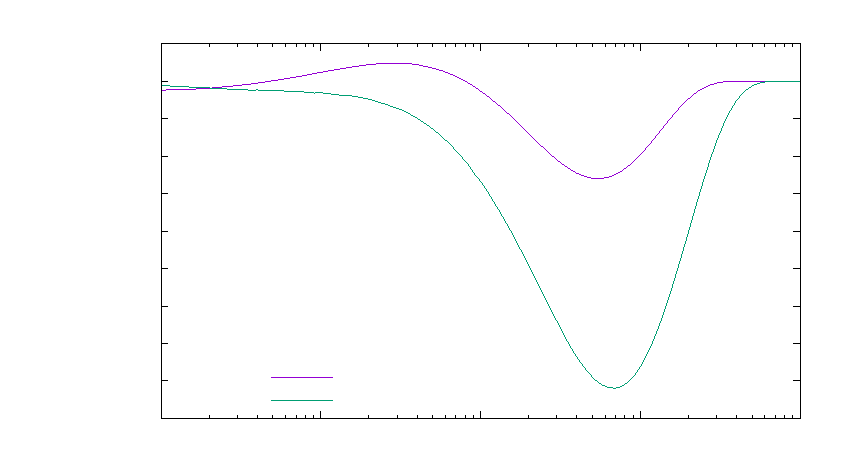
\includegraphics{img/Fq1P}}%
    \gplfronttext
  \end{picture}%
\endgroup

\end{subfigure}
\caption{next-to-leading order hadronic structure functions $F_{k,q}^{(1)}(x,Q^2,m_c^2)$ plotted as function of $x$ for different values of $Q^2$ in units of $\si{\GeV^2}$}\label{fig:Fq1}
\end{figure}

\pagebreak
\begin{figure}[ht!]
\centering
\begin{subfigure}[t]{\textwidth}
	% GNUPLOT: LaTeX picture with Postscript
\begingroup
  \makeatletter
  \providecommand\color[2][]{%
    \GenericError{(gnuplot) \space\space\space\@spaces}{%
      Package color not loaded in conjunction with
      terminal option `colourtext'%
    }{See the gnuplot documentation for explanation.%
    }{Either use 'blacktext' in gnuplot or load the package
      color.sty in LaTeX.}%
    \renewcommand\color[2][]{}%
  }%
  \providecommand\includegraphics[2][]{%
    \GenericError{(gnuplot) \space\space\space\@spaces}{%
      Package graphicx or graphics not loaded%
    }{See the gnuplot documentation for explanation.%
    }{The gnuplot epslatex terminal needs graphicx.sty or graphics.sty.}%
    \renewcommand\includegraphics[2][]{}%
  }%
  \providecommand\rotatebox[2]{#2}%
  \@ifundefined{ifGPcolor}{%
    \newif\ifGPcolor
    \GPcolorfalse
  }{}%
  \@ifundefined{ifGPblacktext}{%
    \newif\ifGPblacktext
    \GPblacktexttrue
  }{}%
  % define a \g@addto@macro without @ in the name:
  \let\gplgaddtomacro\g@addto@macro
  % define empty templates for all commands taking text:
  \gdef\gplbacktext{}%
  \gdef\gplfronttext{}%
  \makeatother
  \ifGPblacktext
    % no textcolor at all
    \def\colorrgb#1{}%
    \def\colorgray#1{}%
  \else
    % gray or color?
    \ifGPcolor
      \def\colorrgb#1{\color[rgb]{#1}}%
      \def\colorgray#1{\color[gray]{#1}}%
      \expandafter\def\csname LTw\endcsname{\color{white}}%
      \expandafter\def\csname LTb\endcsname{\color{black}}%
      \expandafter\def\csname LTa\endcsname{\color{black}}%
      \expandafter\def\csname LT0\endcsname{\color[rgb]{1,0,0}}%
      \expandafter\def\csname LT1\endcsname{\color[rgb]{0,1,0}}%
      \expandafter\def\csname LT2\endcsname{\color[rgb]{0,0,1}}%
      \expandafter\def\csname LT3\endcsname{\color[rgb]{1,0,1}}%
      \expandafter\def\csname LT4\endcsname{\color[rgb]{0,1,1}}%
      \expandafter\def\csname LT5\endcsname{\color[rgb]{1,1,0}}%
      \expandafter\def\csname LT6\endcsname{\color[rgb]{0,0,0}}%
      \expandafter\def\csname LT7\endcsname{\color[rgb]{1,0.3,0}}%
      \expandafter\def\csname LT8\endcsname{\color[rgb]{0.5,0.5,0.5}}%
    \else
      % gray
      \def\colorrgb#1{\color{black}}%
      \def\colorgray#1{\color[gray]{#1}}%
      \expandafter\def\csname LTw\endcsname{\color{white}}%
      \expandafter\def\csname LTb\endcsname{\color{black}}%
      \expandafter\def\csname LTa\endcsname{\color{black}}%
      \expandafter\def\csname LT0\endcsname{\color{black}}%
      \expandafter\def\csname LT1\endcsname{\color{black}}%
      \expandafter\def\csname LT2\endcsname{\color{black}}%
      \expandafter\def\csname LT3\endcsname{\color{black}}%
      \expandafter\def\csname LT4\endcsname{\color{black}}%
      \expandafter\def\csname LT5\endcsname{\color{black}}%
      \expandafter\def\csname LT6\endcsname{\color{black}}%
      \expandafter\def\csname LT7\endcsname{\color{black}}%
      \expandafter\def\csname LT8\endcsname{\color{black}}%
    \fi
  \fi
    \setlength{\unitlength}{0.0500bp}%
    \ifx\gptboxheight\undefined%
      \newlength{\gptboxheight}%
      \newlength{\gptboxwidth}%
      \newsavebox{\gptboxtext}%
    \fi%
    \setlength{\fboxrule}{0.5pt}%
    \setlength{\fboxsep}{1pt}%
\begin{picture}(7920.00,4082.40)%
    \gplgaddtomacro\gplbacktext{%
      \csname LTb\endcsname%
      \put(1254,220){\makebox(0,0)[r]{\strut{} 1.0e+00}}%
      \put(1254,820){\makebox(0,0)[r]{\strut{} 1.5e+00}}%
      \put(1254,1419){\makebox(0,0)[r]{\strut{} 2.0e+00}}%
      \put(1254,2019){\makebox(0,0)[r]{\strut{} 2.5e+00}}%
      \put(1254,2619){\makebox(0,0)[r]{\strut{} 3.0e+00}}%
      \put(1254,3218){\makebox(0,0)[r]{\strut{} 3.5e+00}}%
      \put(1254,3818){\makebox(0,0)[r]{\strut{} 4.0e+00}}%
      \put(1386,0){\makebox(0,0){\strut{}$0.0001$}}%
      \put(2920,0){\makebox(0,0){\strut{}$0.001$}}%
      \put(4454,0){\makebox(0,0){\strut{}$0.01$}}%
      \put(5988,0){\makebox(0,0){\strut{}$0.1$}}%
      \put(7522,0){\makebox(0,0){\strut{}$1$}}%
      \put(1509,1659){\makebox(0,0)[l]{\strut{}(a) $R_{2}(x,Q^2,m_c^2)$}}%
    }%
    \gplgaddtomacro\gplfronttext{%
      \csname LTb\endcsname%
      \put(1518,3645){\makebox(0,0)[l]{\strut{}$Q^2=10^{1}$}}%
      \csname LTb\endcsname%
      \put(1518,3425){\makebox(0,0)[l]{\strut{}$Q^2=10^{2}$}}%
    }%
    \gplbacktext
    \put(0,0){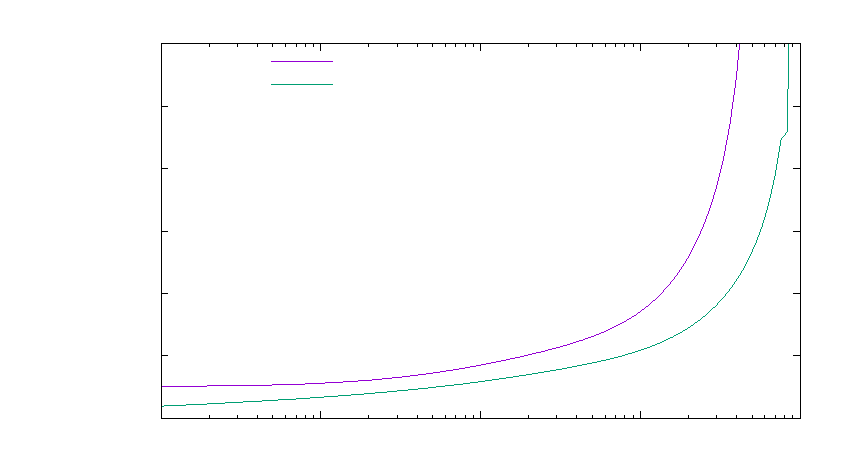
\includegraphics{img/R2}}%
    \gplfronttext
  \end{picture}%
\endgroup

\end{subfigure}\\%
\begin{subfigure}[t]{\textwidth}
	% GNUPLOT: LaTeX picture with Postscript
\begingroup
  \makeatletter
  \providecommand\color[2][]{%
    \GenericError{(gnuplot) \space\space\space\@spaces}{%
      Package color not loaded in conjunction with
      terminal option `colourtext'%
    }{See the gnuplot documentation for explanation.%
    }{Either use 'blacktext' in gnuplot or load the package
      color.sty in LaTeX.}%
    \renewcommand\color[2][]{}%
  }%
  \providecommand\includegraphics[2][]{%
    \GenericError{(gnuplot) \space\space\space\@spaces}{%
      Package graphicx or graphics not loaded%
    }{See the gnuplot documentation for explanation.%
    }{The gnuplot epslatex terminal needs graphicx.sty or graphics.sty.}%
    \renewcommand\includegraphics[2][]{}%
  }%
  \providecommand\rotatebox[2]{#2}%
  \@ifundefined{ifGPcolor}{%
    \newif\ifGPcolor
    \GPcolorfalse
  }{}%
  \@ifundefined{ifGPblacktext}{%
    \newif\ifGPblacktext
    \GPblacktexttrue
  }{}%
  % define a \g@addto@macro without @ in the name:
  \let\gplgaddtomacro\g@addto@macro
  % define empty templates for all commands taking text:
  \gdef\gplbacktext{}%
  \gdef\gplfronttext{}%
  \makeatother
  \ifGPblacktext
    % no textcolor at all
    \def\colorrgb#1{}%
    \def\colorgray#1{}%
  \else
    % gray or color?
    \ifGPcolor
      \def\colorrgb#1{\color[rgb]{#1}}%
      \def\colorgray#1{\color[gray]{#1}}%
      \expandafter\def\csname LTw\endcsname{\color{white}}%
      \expandafter\def\csname LTb\endcsname{\color{black}}%
      \expandafter\def\csname LTa\endcsname{\color{black}}%
      \expandafter\def\csname LT0\endcsname{\color[rgb]{1,0,0}}%
      \expandafter\def\csname LT1\endcsname{\color[rgb]{0,1,0}}%
      \expandafter\def\csname LT2\endcsname{\color[rgb]{0,0,1}}%
      \expandafter\def\csname LT3\endcsname{\color[rgb]{1,0,1}}%
      \expandafter\def\csname LT4\endcsname{\color[rgb]{0,1,1}}%
      \expandafter\def\csname LT5\endcsname{\color[rgb]{1,1,0}}%
      \expandafter\def\csname LT6\endcsname{\color[rgb]{0,0,0}}%
      \expandafter\def\csname LT7\endcsname{\color[rgb]{1,0.3,0}}%
      \expandafter\def\csname LT8\endcsname{\color[rgb]{0.5,0.5,0.5}}%
    \else
      % gray
      \def\colorrgb#1{\color{black}}%
      \def\colorgray#1{\color[gray]{#1}}%
      \expandafter\def\csname LTw\endcsname{\color{white}}%
      \expandafter\def\csname LTb\endcsname{\color{black}}%
      \expandafter\def\csname LTa\endcsname{\color{black}}%
      \expandafter\def\csname LT0\endcsname{\color{black}}%
      \expandafter\def\csname LT1\endcsname{\color{black}}%
      \expandafter\def\csname LT2\endcsname{\color{black}}%
      \expandafter\def\csname LT3\endcsname{\color{black}}%
      \expandafter\def\csname LT4\endcsname{\color{black}}%
      \expandafter\def\csname LT5\endcsname{\color{black}}%
      \expandafter\def\csname LT6\endcsname{\color{black}}%
      \expandafter\def\csname LT7\endcsname{\color{black}}%
      \expandafter\def\csname LT8\endcsname{\color{black}}%
    \fi
  \fi
    \setlength{\unitlength}{0.0500bp}%
    \ifx\gptboxheight\undefined%
      \newlength{\gptboxheight}%
      \newlength{\gptboxwidth}%
      \newsavebox{\gptboxtext}%
    \fi%
    \setlength{\fboxrule}{0.5pt}%
    \setlength{\fboxsep}{1pt}%
\begin{picture}(7920.00,4082.40)%
    \gplgaddtomacro\gplbacktext{%
      \csname LTb\endcsname%
      \put(1254,220){\makebox(0,0)[r]{\strut{} 1.0e+00}}%
      \put(1254,820){\makebox(0,0)[r]{\strut{} 1.5e+00}}%
      \put(1254,1419){\makebox(0,0)[r]{\strut{} 2.0e+00}}%
      \put(1254,2019){\makebox(0,0)[r]{\strut{} 2.5e+00}}%
      \put(1254,2619){\makebox(0,0)[r]{\strut{} 3.0e+00}}%
      \put(1254,3218){\makebox(0,0)[r]{\strut{} 3.5e+00}}%
      \put(1254,3818){\makebox(0,0)[r]{\strut{} 4.0e+00}}%
      \put(1386,0){\makebox(0,0){\strut{}$0.0001$}}%
      \put(2920,0){\makebox(0,0){\strut{}$0.001$}}%
      \put(4454,0){\makebox(0,0){\strut{}$0.01$}}%
      \put(5988,0){\makebox(0,0){\strut{}$0.1$}}%
      \put(7522,0){\makebox(0,0){\strut{}$1$}}%
      \put(1509,1659){\makebox(0,0)[l]{\strut{}(b) $R_{L}(x,Q^2,m_c^2)$}}%
    }%
    \gplgaddtomacro\gplfronttext{%
      \csname LTb\endcsname%
      \put(1518,3645){\makebox(0,0)[l]{\strut{}$Q^2=10^{1}$}}%
      \csname LTb\endcsname%
      \put(1518,3425){\makebox(0,0)[l]{\strut{}$Q^2=10^{2}$}}%
    }%
    \gplbacktext
    \put(0,0){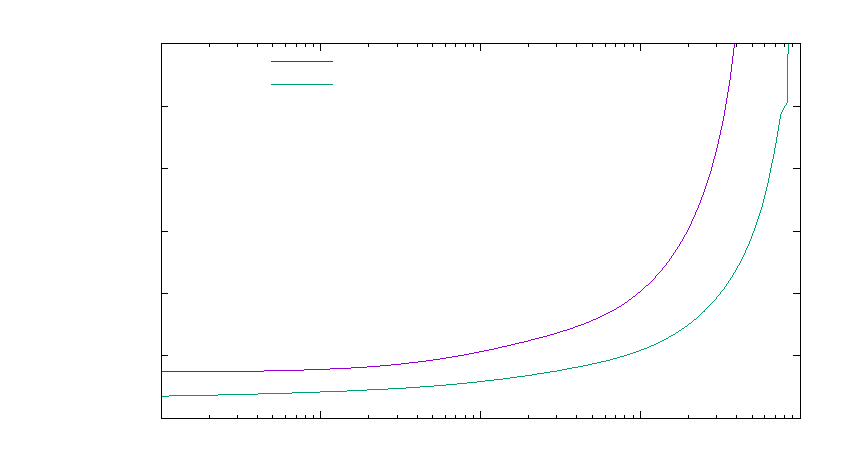
\includegraphics{img/RL}}%
    \gplfronttext
  \end{picture}%
\endgroup

\end{subfigure}\\%
\begin{subfigure}[t]{\textwidth}
	% GNUPLOT: LaTeX picture with Postscript
\begingroup
  \makeatletter
  \providecommand\color[2][]{%
    \GenericError{(gnuplot) \space\space\space\@spaces}{%
      Package color not loaded in conjunction with
      terminal option `colourtext'%
    }{See the gnuplot documentation for explanation.%
    }{Either use 'blacktext' in gnuplot or load the package
      color.sty in LaTeX.}%
    \renewcommand\color[2][]{}%
  }%
  \providecommand\includegraphics[2][]{%
    \GenericError{(gnuplot) \space\space\space\@spaces}{%
      Package graphicx or graphics not loaded%
    }{See the gnuplot documentation for explanation.%
    }{The gnuplot epslatex terminal needs graphicx.sty or graphics.sty.}%
    \renewcommand\includegraphics[2][]{}%
  }%
  \providecommand\rotatebox[2]{#2}%
  \@ifundefined{ifGPcolor}{%
    \newif\ifGPcolor
    \GPcolorfalse
  }{}%
  \@ifundefined{ifGPblacktext}{%
    \newif\ifGPblacktext
    \GPblacktexttrue
  }{}%
  % define a \g@addto@macro without @ in the name:
  \let\gplgaddtomacro\g@addto@macro
  % define empty templates for all commands taking text:
  \gdef\gplbacktext{}%
  \gdef\gplfronttext{}%
  \makeatother
  \ifGPblacktext
    % no textcolor at all
    \def\colorrgb#1{}%
    \def\colorgray#1{}%
  \else
    % gray or color?
    \ifGPcolor
      \def\colorrgb#1{\color[rgb]{#1}}%
      \def\colorgray#1{\color[gray]{#1}}%
      \expandafter\def\csname LTw\endcsname{\color{white}}%
      \expandafter\def\csname LTb\endcsname{\color{black}}%
      \expandafter\def\csname LTa\endcsname{\color{black}}%
      \expandafter\def\csname LT0\endcsname{\color[rgb]{1,0,0}}%
      \expandafter\def\csname LT1\endcsname{\color[rgb]{0,1,0}}%
      \expandafter\def\csname LT2\endcsname{\color[rgb]{0,0,1}}%
      \expandafter\def\csname LT3\endcsname{\color[rgb]{1,0,1}}%
      \expandafter\def\csname LT4\endcsname{\color[rgb]{0,1,1}}%
      \expandafter\def\csname LT5\endcsname{\color[rgb]{1,1,0}}%
      \expandafter\def\csname LT6\endcsname{\color[rgb]{0,0,0}}%
      \expandafter\def\csname LT7\endcsname{\color[rgb]{1,0.3,0}}%
      \expandafter\def\csname LT8\endcsname{\color[rgb]{0.5,0.5,0.5}}%
    \else
      % gray
      \def\colorrgb#1{\color{black}}%
      \def\colorgray#1{\color[gray]{#1}}%
      \expandafter\def\csname LTw\endcsname{\color{white}}%
      \expandafter\def\csname LTb\endcsname{\color{black}}%
      \expandafter\def\csname LTa\endcsname{\color{black}}%
      \expandafter\def\csname LT0\endcsname{\color{black}}%
      \expandafter\def\csname LT1\endcsname{\color{black}}%
      \expandafter\def\csname LT2\endcsname{\color{black}}%
      \expandafter\def\csname LT3\endcsname{\color{black}}%
      \expandafter\def\csname LT4\endcsname{\color{black}}%
      \expandafter\def\csname LT5\endcsname{\color{black}}%
      \expandafter\def\csname LT6\endcsname{\color{black}}%
      \expandafter\def\csname LT7\endcsname{\color{black}}%
      \expandafter\def\csname LT8\endcsname{\color{black}}%
    \fi
  \fi
    \setlength{\unitlength}{0.0500bp}%
    \ifx\gptboxheight\undefined%
      \newlength{\gptboxheight}%
      \newlength{\gptboxwidth}%
      \newsavebox{\gptboxtext}%
    \fi%
    \setlength{\fboxrule}{0.5pt}%
    \setlength{\fboxsep}{1pt}%
\begin{picture}(7920.00,4082.40)%
    \gplgaddtomacro\gplbacktext{%
      \csname LTb\endcsname%
      \put(1254,220){\makebox(0,0)[r]{\strut{}-2.0e+00}}%
      \put(1254,670){\makebox(0,0)[r]{\strut{}-1.5e+00}}%
      \put(1254,1120){\makebox(0,0)[r]{\strut{}-1.0e+00}}%
      \put(1254,1569){\makebox(0,0)[r]{\strut{}-5.0e-01}}%
      \put(1254,2019){\makebox(0,0)[r]{\strut{}0.0e+00}}%
      \put(1254,2469){\makebox(0,0)[r]{\strut{}5.0e-01}}%
      \put(1254,2919){\makebox(0,0)[r]{\strut{}1.0e+00}}%
      \put(1254,3368){\makebox(0,0)[r]{\strut{}1.5e+00}}%
      \put(1254,3818){\makebox(0,0)[r]{\strut{}2.0e+00}}%
      \put(1386,0){\makebox(0,0){\strut{}$0.0001$}}%
      \put(2920,0){\makebox(0,0){\strut{}$0.001$}}%
      \put(4454,0){\makebox(0,0){\strut{}$0.01$}}%
      \put(5988,0){\makebox(0,0){\strut{}$0.1$}}%
      \put(7522,0){\makebox(0,0){\strut{}$1$}}%
      \put(1509,1659){\makebox(0,0)[l]{\strut{}(c) $R_P(x,Q^2,m_c^2)$}}%
    }%
    \gplgaddtomacro\gplfronttext{%
      \csname LTb\endcsname%
      \put(1518,3645){\makebox(0,0)[l]{\strut{}$Q^2=10^{1}$}}%
      \csname LTb\endcsname%
      \put(1518,3425){\makebox(0,0)[l]{\strut{}$Q^2=10^{2}$}}%
    }%
    \gplbacktext
    \put(0,0){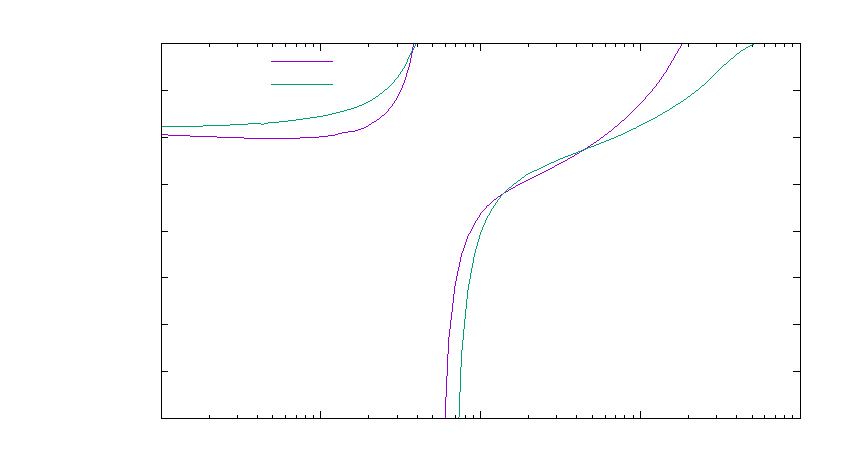
\includegraphics{img/RP}}%
    \gplfronttext
  \end{picture}%
\endgroup

\end{subfigure}
\caption{ratio of hadronic structure functions $R_{k'}^{(1)}(x,Q^2,m_c^2)$ plotted as function of $x$ for different values of $Q^2$ in units of $\si{\GeV^2}$}\label{fig:R}
\end{figure}

\clearpage
\pagebreak
